%%% compile it with pdflatex
\documentclass[a4paper]{article}
\usepackage[T1]{fontenc}
\usepackage[utf8]{inputenc}
\usepackage{lmodern}
\usepackage{fancybox}
\usepackage{graphicx}
\usepackage{tabularx}

\begin{document}

\title{2APL: A Practical Programming Language and Platform for Multi-Agent Systems}
 
\author{Beltran Borja Fiz, Fabrizio De Santis, Marcos Gabarda\\
\small \texttt{\{beltran.borja.fiz, fabrizio.de.santis, marcos.gabarda\}@est.fib.upc.edu}\\
\\
Multi-Agent Systems Course\\
Master in Artificial Intelligence\\
Universitat Polit\`ecnica de Catalunya}
\date{\today}

\newenvironment{fminipage}%
  {\begin{Sbox}\begin{minipage}}%
  {\end{minipage}\end{Sbox}\fbox{\TheSbox}}


\maketitle

\tableofcontents

\section{Introduction} %%%%%%% BORJA HERE

The 2APL (pronounced double-a-p-l) Platform is a development tool that is designed to support the implementation and execution of multi-agent systems programmed in 2APL Language. 2APL has been designed and developed at the Intelligent Systems Group at the University of Utrecht. 2APL language is a BDI-based agent-oriented programming language that supports an integration of declarative programming constructs such as belief and goals and imperative style programming constructs such as events and plans. The 2APL platform
provides a graphical interface through which a programmer can develop and execute 2APL multi-agent systems using several facilities. The platform allows communication among agents and can run on several machines connected in a network.
In section~\ref{sec:lang} we will introduce the 2APL language describing its syntax, operational and formal semantics for specifying a multi-agent system and individual agents. Also, the deliberation cycle will be discussed. In section~\ref{sec:platform} we will discuss the 2APL Platform ...


\section{2APL Language}\label{sec:lang} %%%%%%% BORJA HERE 

2APL language is a BDI-based agent-oriented programming language that realizes an integration of declarative and imperative style programming. The declarative style programming supports the implementation of the mental state of agents allowing them to reason about their mental states and update them accordingly. The imperative style programming supports the implementation of  processes allowing programming constructs to implement both the flow of control as well as mechanisms such as procedure call, recursion, plan revision, and interface to existing imperative programming languages. In this section, we will proceed illustrating the syntax of the language and both the operational and formal semantics. We will conclude the section discussing the execution of a multi-agent system and the 2APL deliberation process.

\subsection{Syntax and operational semantics} %%%%%%% FABRIZIO HERE

There are 2 distinguished set of programming constructs for specifying a multi-agent system and individual agents. Our approach will be to illustrate the formal syntax little by little providing the explanation of operational semantics through simple fragments of code.

\subsubsection{Multi-agent system specification} %%%%%%% FABRIZIO HERE

A multi-agent system is specified as a set of couples, each of them, specifying an agent of the society and a set of environments it has access to. The formal syntax for specifying a multi-agent system is provided in Figure~\ref{fig:ebnf_mas}. 

\begin{figure}[htbp]
\begin{verbatim}
<MAS_Prog>     := ( <agentname> ``:'' <filename> [<int>]
                   [<environments>] )+
<agentname>    := <ident>
<filename>     := <ident>``.2apl''
<environments> := ``@''<ident> (``,'' <ident>)*
\end{verbatim}
\caption{EBNF syntax for specifying a multi-agent system}
\label{fig:ebnf_mas}
\end{figure}

Figure~\ref{fig:ex_blockworld} shows an example of a multi-agent system where there are defined two agents, \texttt{harry} and \texttt{sally}, both having access to the same environment called \texttt{blockWorld}.

\begin{figure}[htbp]
\begin{verbatim}
harry : harry.2apl @blockworld
sally : sally.2apl @blockworld
\end{verbatim}
\caption{Example of a multi-agent system specification}
\label{fig:ex_blockworld}
\end{figure}

\subsubsection{Individual agent specification} %%%%%%% FABRIZIO HERE

% 
% Agent can observe an environment either:
% \begin{itemize}
%   \item actively by means of a sense action
%   \item passively by means of events generated by the environment
% \end{itemize}

Basically, 2APL agents are implemented in terms of beliefs, goals, actions, plans, events and three different kind of practical reasoning rules in order to generate plans for achieving goals, processing events or messages and for handling and repairing failed plans. Figure~\ref{fig:ebnf_agent} provides the formal syntax for specifying an individual agent in such terms.

\begin{figure}[htp]
\begin{verbatim}
	<Agent_Prog> := ( ``Include:'' <ident>
	                | ``BeliefUpdates:'' <BelUpSpec>
	                | ``Beliefs:'' <belief> 
	                | ``Goals:'' <goals> 
	                | ``Plans:'' <plans>
	                | ``PG-rules:'' <pgrules>
	                | ``PC-rules:'' <pcrules>
	                | ``PR-rules:'' <prrules>
	                )*
\end{verbatim}
\caption{EBNF syntax for specifying an individual agent}
\label{fig:ebnf_agent}
\end{figure}

The basic building elements of the language are \texttt{<atom>} that denotes a Prolog like atomic formula starting with a lowercase letter used for stating Prolog atomic formulas, \texttt{<Atom>} that, again, denotes a Prolog like atomic formula starting with a capital letter but, in this case, it is used for invoking functions, \texttt{<ground\_atom>} that denotes a Prolog ground atomic formula\footnote{Prolog formula that does not contain variables}, \texttt{<Var>} that denotes as a string with a capital letter and it is used for variables and, finally, \texttt{<ident>} that denotes a string with a lowercase letter and it used for identifiers.

\paragraph{Beliefs and Goals}

A 2APL agent has \emph{beliefs} and \emph{goals} that usually change during the execution. The initial set of beliefs and goals are defined specifying a \emph{belief base} and a \emph{goal base}. As a principle of rationality we should assume that if an agent believes a certain fact, then it can not purse that fact as a goal. This assumption put on evidence that there is a link between the two bases: if an agent modifies its belief base, then its goal base may require a modification as well. 

The formal syntax for specifying a belief base is provided in Figure~\ref{fig:ebnf_beliefbase}. 

\begin{figure}[htp]
\begin{verbatim}
	``Beliefs:'' <belief>
	
	<belief>   := ( <ground_atom> ``.''
	              | <atom> ``:-'' <literals> ``.'' 
	              )+
	<literals> := <literal> (``,'' <literal>)*
	<literal>  := ( <atom> 
	              | ``not'' <atom>
	              )
	\end{verbatim}
\caption{EBNF syntax for specifying a belief base}
\label{fig:ebnf_beliefbase}
\end{figure}

Figure~\ref{fig:example_beliefbase} shows an example of a belief base for an agent that believes that there is a bomb at position $(3,4)$ and that \texttt{blockWorld} environment is clean if does contain no bombs anymore and the agent itself is not carrying a bomb. Actually, looking back to the basic elements of the language, it can be easy to realize that a belief base is a Prolog program where each belief is either a Prolog rule or fact that must be ground.

\begin{figure}[htp]
\begin{verbatim}
Beliefs:
       bomb(3,4).
       clean(blockWorld) :- not bomb(X,Y), not carry(bomb).
\end{verbatim}
\caption{Example of a belief base}
\label{fig:example_beliefbase}
\end{figure}

Analogously, Figure~\ref{fig:ebnf_goalbase} provides the formal syntax for specifying a goal base and Figure~\ref{fig:example_goalbase} shows an example in which the agent has the goal of achieving a situation in which the \texttt{blockWorld} environment is clean. %Each goal expression is a conjunction of ground atoms. 

\begin{figure}[htp]
\begin{verbatim}
``Goals:'' <goals>

<goals> := <goal> ( ``,'' <goal> )*
<goal>  := <ground_atom> ( ``and'' <ground_atom> )*
\end{verbatim}
\caption{EBNF syntax for specifying a goal base}
\label{fig:ebnf_goalbase}
\end{figure}

\begin{figure}[htp]
\begin{verbatim}
Goals:
     clean(blockWorld)
\end{verbatim}
\caption{Example of a goal base}
\label{fig:example_goalbase}
\end{figure}

It is worth noting that having a goal ``\texttt{a and b}'' is different than having two goals ``\texttt{a, b}''. In the former the agent is pursuing the goal of achieving both the goal \texttt{a} and the goal \texttt{b} together, while in the latter the agent has two different goals \texttt{a} and \texttt{b} to achieve. Moreover, it is important to state that a goal base is actually an ordered list such that the goals are ordered by a priority. The first goal in the list is the one with highest priority, while the last goal in the list is the one with the lowest priority.

\paragraph{Basic Actions}

A 2APL agent may choose among 6 types of basic actions in order to achieve its goals: belief base update action, communication action, external action, abstract action, test actions and goal dynamic actions. The formal syntax for specifying actions is provided in Figure~\ref{fig:ebnf_actions}.

\begin{figure}[htp]
\begin{verbatim}
<baction> = ( <beliefupdate>
            | <sendaction> | <externalaction> 
            | <abstractaction> | <test>
            | <adoptgoal> | <dropgoal>
            )
\end{verbatim}
\caption{EBNF syntax for specifying basic actions}
\label{fig:ebnf_actions}
\end{figure}

A \emph{belief update action} updates the belief base exploiting the \emph{precondition-delete-add} formalism. An agent can
execute a belief update action if the precondition of the action is entailed by its belief base. The execution of the action then modifies the belief base in such a way that after the execution the post-condition of the action is derivable from the belief base. It is worth noting that the execution of a belief base has as side-effect that goals that become believed to be achieved are removed. The formal syntax of a \emph{belief base update action} is provided in Figure~\ref{fig:ebnf_beliefupdate}.

\begin{figure}[htp]
\begin{verbatim}
	``BeliefUpdates:'' <BelUpSpec>
	
	<BelUpSpec>    := (
	                  ``{'' <belquery> ``}''
	                      <beliefupdate>
	                  ``{'' <literals> ``}''
	                  )+
	<belquery>     := ( ``true'' 
	                  | <belquery> ``and'' <belquery>
	                  | <belquery> ``or'' <belquery>
	                  | ``('' <belquery> ``)''
	                  | <literal>
	                  )
	<beliefupdate> := <Atom>
\end{verbatim}
\caption{EBNF syntax for specifying belief update action}
\label{fig:ebnf_beliefupdate}
\end{figure}

Figure~\ref{fig:example_beliefupdate} provides an excerpt of belief update actions available in agent \texttt{harry}. For instance, the agent can pickup a bomb if the agent believes it does not already carrying a bomb and, if the action will succeed, the agent will believe that it is carrying a bomb. %It important to see that the agent cannot pickup a bomb consecutively.

\begin{figure}[htp]
\begin{verbatim}
BeliefUpdates:
  { bomb(X,Y) }       RemoveBomb(X,Y) { not bomb(X,Y) }
  { true }            AddBomb(X,Y)    { bomb(X,Y) }
  { carry(bomb) }     Drop()          { not carry(bomb) }
  { not carry(bomb) } PickUp()        { carry(bomb) }
\end{verbatim}
\caption{Example of belief update actions}
\label{fig:example_beliefupdate}
\end{figure}

A \emph{communication action} is used to pass a message to other agents. Figure~\ref{fig:ebnf_sendaction} provides the formal specification of the action. Let consider the action \texttt{send(harry, inform, La, On, bombAt(X\_1, Y\_1)}. In this case, the agent \texttt{sally} is sending a message to the agent \texttt{harry} using the perfomative of informing him that there is a bomb at position $(X_1, Y_1)$ using the content language \texttt{La} and the ontology \texttt{On}.

\begin{figure}[htp]
\begin{verbatim}
<sendaction> := ``send('' <iv> ``,'' <iv> ``,''
                        [ <iv> ``,'' <iv> ``,'' ]  <atom> ``)''  
<iv>         := <ident> | <Var>
\end{verbatim}
\caption{EBNF syntax for specifying send action}
\label{fig:ebnf_sendaction}
\end{figure}

Actually, a send action can be also performed omitting the specification of the content language and ontology, if it reasonable to assume that all the agents in system share the same content language and ontologies.

An \emph{external action} is supposed to change the state of an external environment. The effects of external actions are, in fact, assumed to be determined by the environment. Thus, a sense action (that is also an external action) has to be performed in order to determine the effect of a previous external action. The formal syntax is provided in Figure~\ref{fig:ebnf_extaction}. An example of external actions is \texttt{@blockworld(east(), L)} that would try to get the agent one step to the east in the \texttt{blockWorld} environment.

\begin{figure}[htp]
\begin{verbatim}
<externalaction> := ``@'' <ident> ``('' <atom> ``,'' <Var> ``)''
\end{verbatim}
\caption{EBNF syntax for specifying external action}
\label{fig:ebnf_extaction}
\end{figure}

An \emph{abstract action} is used to instantiate a new plan when the action is executed in the way a procedure call would instantiate a new procedure. The formal syntax is provided in Figure~\ref{fig:ebnf_absaction}. A example of this action will be shown later in a concrete scenario.

\begin{figure}[htp]
\begin{verbatim}
<abstractaction> := <atom>
\end{verbatim}
\caption{EBNF syntax for specifying abstract action}
\label{fig:ebnf_absaction}
\end{figure}

\emph{Test actions} are query expressions used to check if an agent can derive certain beliefs and goals from its bases. The formal syntax is provided in Figure~\ref{fig:ebnf_testaction}.

\begin{figure}[htp]
\begin{verbatim}
<test>      := ( ``B('' <belquery> ``)'' 
               | ``G('' <goalquery> ``)''
               | <test> ``&'' <test>
               )
<goalquery> := ( ``true'' 
               | <goalquery> ``and'' <goalquery>
               | <goalquery> ``or'' <goalquery>
               | ``('' <goalquery> ``)''
               | <atom>
               )
\end{verbatim}
\caption{EBNF syntax for specifying test actions}
\label{fig:ebnf_testaction}
\end{figure}

Let imagine that, for instance, an agent has a certain belief \texttt{p(a)} and it is  pursing the goal of achieving a situation \texttt{q(b)} and we are querying first for \texttt{B(p(X)) \& G(q(X))} and then for \texttt{B(p(X)) \& G(q(Y) or r(X))}. In the first case the query will fail since no substitution is possible, while in the second case the query will succeed by the substitution $\rho=\{X/a, Y/b\}$.

\emph{Goal dynamics action} are used to adopt and drop goals to and from an agent's goal base. The adopt goal action has two forms, the first one for adopting a goal giving it the maximum priority and another one for giving it the least priority. Also, the drop goal action has three different forms they are used to drop from an agent’s goal base, respectively, exactly the goal specified, all goals that are subgoal of the goal specified and all goals that have the goal specified as a subgoal. The formal syntax is provided in Figure~\ref{fig:ebnf_goalactions}.

\begin{figure}[htp]
\begin{verbatim}
<adoptgoal> := ( ``adopta('' <goalvar> ``)''
               | ``adoptz('' <goalvar> ``)''
               )
<dropgoal>  := ( ``dropgoal('' <goalvar> ``)''
               | ``dropsubgoals('' <goalvar> ``)''
               | ``dropsupergoals('' <goalvar> ``)''
               )
<goalvar>   := ( <atom> | ``not'' <atom> )
\end{verbatim}
\caption{EBNF syntax for specifying goal dynamics actions}
\label{fig:ebnf_goalactions}
\end{figure}

To illustrate the use of these three different actions to drop a goal the following three goals are considered: \texttt{a(1), a(1) and b(1), a(1) and b(1)}. Then a \texttt{dropgoal(a(1) and b(1))} action will drop exactly the \texttt{a(1) and b(1)}, the \texttt{dropsubgoal(a(1) and b(1))} will drop the goal \texttt{a(1) and b(1)} and its subgoal \texttt{a(1)} and, finally, the action \texttt{dropsupergoal(a(1) and b(1))} will drop the goal \texttt{a(1) and b(1)} and its supergoal \texttt{a(1) and b(1) and c(1)}.

\paragraph{Plans}

In order to reach its goals, a agent needs to adopt \emph{plans}. A plan consists of basic actions that can be composed by using the following operators: sequence operator, conditional choice operators, conditional iteration operator and atomic operator for plans that must be executed atomically. The formal syntax for both specifying a plan and a plan base is provided in Figure~\ref{fig:ebnf_plans}.

\begin{figure}[htp]
\begin{verbatim}
<plan>         := ( <baction> | <sequenceplan>
                  | <ifplan> | <whileplan>
                  | <atomicplan>
                  )
<sequenceplan> := <plan> ``;'' <plan>
<ifplan>       := ``if'' <test> ``then'' <scopeplan>
                 [``else'' <scopeplan>]
<scopeplan>    := ``{'' <plan ``}''
<whileplan>    := ``while'' <text> ``do'' <scopeplan>
<atomicplan>   := ``['' <plan> ``]''

Plans: <plans>
       <plans> := <plan> ( ``,'' <plan> )*
\end{verbatim}
\caption{EBNF syntax for specifying plans and a plan base}
\label{fig:ebnf_plans}
\end{figure}

Figure~\ref{fig:ebnf_planbase} shows an example of the implementation of an initial plan base of \texttt{harry} that let him enter the \texttt{blockWorld} environment by performing a test action and then an external action. It worth noting that during execution of the agent, the plan base will be filled with plans by means of reasoning rules.
 
\begin{figure}[htp]
\begin{verbatim}
Plans:
	B(start(X,Y)) ; @blockworld(enter(X, Y, blue), L)
\end{verbatim}	
\caption{Example of a plan base}
\label{fig:ebnf_planbase}
\end{figure}

\paragraph{Reasoning Rules}

There are three kind of \emph{practical reasoning rules} that are used to implement the generation of plans: planning goal rules (PG rules), procedural rules (PC rules) and plan repair rules (PR rules). 

PG rules are used to generate plans starting from certain beliefs and goals. The formal syntax is provided in Figure~\ref{fig:ebnf_pgrules}.

\begin{figure}[htp]
\begin{verbatim}
``PG-rules:'' <pgrules>

<pgrules> := <pgrule>+
<pgrule>  := [<goalquery>] ``<-'' <belquery> ``|'' <plan>
\end{verbatim}
\caption{EBNF syntax for specifying PG rules}
\label{fig:ebnf_pgrules}
\end{figure}

An example of a planning goal rule is provided in Figure~\ref{fig:example_pgrules} indicating that a plan to achieve the goal \texttt{clean(blockWorld)} can be generated if the agent believes there is a bomb at position $(X,Y)$. Note that \texttt{goto(X,Y)} is an example of abstract action, \texttt{@blockworld(pickup(), L1)} is an external action and \texttt{PickUp()} is a belief update action.

\begin{figure}[htp]
\begin{verbatim}
PG-rules:
clean(blockWorld) <- bomb(X, Y) | { 
goto(X, Y);
@blockworld(pickup(), L1);
PickUp();
RemoveBomb(X, Y);

goto(0, 0);
@blockworld(drop(), L2);
Drop();
}
\end{verbatim}
\caption{Example of PG rules}
\label{fig:example_pgrules}
\end{figure}

PC rules are used to generate plans as a response to the execution of abstract actions or the reception of messages from other agents or events generated from the environment. A procedural rule is applied if and only if the belief condition is entailed by the belief base. The formal syntax is provided in Figure~\ref{fig:ebnf_pcrules}.

\begin{figure}[htp]
\begin{verbatim}
``PC-rules:'' <pcrules>

<pcrules> = <pcrule>+
<pcrule> = <atom> ``<-'' <belquery> ``|'' <plan>
\end{verbatim}
\caption{EBNF syntax for specifying PC rules}
\label{fig:ebnf_pcrules}
\end{figure}

Figure~\ref{fig:example_pcrules} shows an example of two procedural rules for \texttt{harry}, the first one indicating that the abstract action \texttt{goto} is actually a certain sequence of actions, while second one indicating that if \texttt{harry} receives a message from \texttt{sally} informing him that there is a bomb at position $(X,Y)$ and \texttt{harry} does not believe there are any bombs, then harry updates his beliefs with this new fact and adds a goal to clean the \texttt{blockWorld} again.

\begin{figure}[htp]
\begin{verbatim}
PC-rules:
goto(X, Y) <- true | {
  @blockworld(sensePosition(), POS);
  B(POS = [A,B]);
  if B(A > X) then {
     @blockworld( west(), L);
     goto(X, Y);
  } else if B(A < X) then {
     @blockworld( east(), L);
     goto(X, Y);
  } else if B(B > Y) then {
     @blockworld( north(), L);
     goto(X, Y);
  } else if B(B < Y) then {
    @blockworld(south(), L);
    goto(X, Y);
  }
}

message(sally, inform, La, On, bombAt(X, Y)) <- true | {
	  if B(not bomb(A, B)) then { 
	    AddBomb(X, Y);
	    adoptz(clean(blockWorld));
	  } else { 
	    AddBomb(X, Y);
	  }
	}
\end{verbatim}
\caption{Example of two kinds of PC rules}
\label{fig:example_pcrules}
\end{figure}

Finally, PR rules are used to replace a plan whose execution has failed. Plan repair rules can be applied if the following condition hold: the execution of a plan fails, there is a rule matching the failed action and the belief query expression is derivable from the agent's belief base. The formal syntax of PR rules is provided in Figure~\ref{fig:ebnf_prrules}.

\begin{figure}[htp]
\begin{verbatim}
``PR-rules:'' <prrules>
<prrules>      := <prrule>+
<pcrule>       := <planvar> ``<-'' <belquery> ``|'' <planvar>
<planvar>      := ( <plan>
                  | <Var>
                  | ``if'' <test> ``then'' <scopeplanvar>
                   [``else'' <scopeplanvar>]
                  | ``while'' <test> ``do'' <scopeplanvar> 
                  | <planvar> ``;'' <planvar>
                  )
<scopeplanvar> := ``{'' <planvar> ``}''
\end{verbatim}
\caption{EBNF syntax for specifying PR rules}
\label{fig:ebnf_prrules}
\end{figure}

An example of a plan repair rule of \texttt{harry} is shown in Figure~\ref{fig:example_pcrules}. This rule is used for the situation in which the execution of a plan that starts with the external action \texttt{@blockworld(pickup(),L)} fails. Such an action fails in case there is no bomb to be picked up, may be because it has already been removed by another agent. The rule states that the plan should be replaced by a plan in which the agent updates its beliefs about the location of the bombs. It is worth noting that the rest of the original plan denoted by \texttt{REST} is dropped, as it is not used anymore within the rule.

\begin{figure}[htp]
\begin{verbatim}
PR-rules:
@blockworld(pickup(), L) ; REST <- true | { 
  @blockworld(sensePosition(), POS);
  B(POS = [X, Y]);     // test action	
  RemoveBomb(X, Y);    // belief update action
}
\end{verbatim}
\caption{Example of two kinds of PC rules}
\label{fig:example_pcrules}
\end{figure}

Finally, it is important to see that the execution of a plan fails if the execution of its first action fail and, when an action fails, depends on the type of the action. Table~\ref{table:action_fail} provides a quick summary of possible causes for each kind of action.

\begin{table}[htp]
  \begin{tabular}{|l| p{8.5cm}|}
  \hline
  Belief update action & It is not specified or the pre-condition is not entailed by the belief base  \\
  \hline
  Abstract action & There is no applicable procedural rule \\
  \hline
  External action & The environment throws an \texttt{ExternalActionFailedException},the agent has no access to the environment, the actions is not defined in the environment \\
  \hline
  Test action & The test expression is no derivable from the belief or goal bases \\
  \hline
  Goal adopt action & The goal is already entailed by the belief base, the goal to be adopted is not ground\\
  \hline
  Atomic plan & If one of its actions fails \\
  \hline
  \end{tabular}
  \caption{Possible causes of failure}
  \label{table:action_fail}
\end{table}

\subsubsection{Programming the environment} %%%%%%% FABRIZIO HERE

A 2APL environment can be any Java class implementing the \emph{environment interface} that contains the following two methods: \texttt{addAgent(String name)} and \texttt{removeAgent(String name)}. Any external action like \texttt{@env($a_1, \ldots, a_n$, R)} is translated into a call to a method $m$ with arguments $a_1, \ldots, a_n$ in environment $env$. Java exceptions are the mechanisms used to inform an agent that an execution of an action has failed and let it apply plan repair rules. Figure~\ref{fig:example_env} provide an example of a \texttt{move} external action that can fail if an unknown direction is specified.

\begin{figure}[htp]
\begin{verbatim}
public Term move(String agent, String direction)
   throws ExternalActionFailedException {
  	   
   if (direction.equals("north") { moveNorth(); }
   	   else if (direction.equals("east") {moveEast(); }
   	   else if (direction.equals("south") {moveSouth(); }
   	   else if (direction.equals("west") {moveWest(); }
   	   else throw
        new ExternalActionFailedException("Unknown direction");
   	   return getPositionTerm();
}
\end{verbatim}
\caption{Example of}
\label{fig:example_env}
\end{figure}

Finally, it is important to state that the constructor of the environment must require exactly one parameter of the type \texttt{ExternalEventListener}. Such class has the method \texttt{notifyEvent(AF event, String... agents)} that can be used to notify agents of events from the environment. The first argument of this method may be any valid atomic formula. The rest of the arguments may be filled with strings that represent local names of agents. If the programmer does not specify any agents in the argument list, all agents can receive the event. 

\subsection{Formal Semantics} %%%%%%% MARCOS HERE

In this section we present the formal semantics of 2APL in terms of transition system. A transition system is a set of transition rules for deriving transitions. A transitionis is a transformation of one configuration into another and it corresponds to a simple computation/execution step.

The execution of a 2APL multi-agent program modifies its initial configuration by means of transitions that are derivable from the transition rules. In fact, each transition rule indicates which execution step (i.e., transition) is possible from a given configuration. It should be noted that for a given configuration there may be
several transition rules applicable. An interpreter is a deterministic choice of applying transition rules in a certain order.

\subsubsection{2APL Configurations}

The configuration of an individual agent consists of its \textbf{identifier}, \textbf{beliefs}, \textbf{goals}, \textbf{plans}, \textbf{substitutions that are resulted from queries to the belief and goal bases}, and the \textbf{received events}. Moreover, additional information is assigned to an agent's plan. In particular, a unique identifier is assigned to each plan which can be used to identify and repair failed plans. Also, the practical reasoning rules by means of which plans are generated are assigned to plans in order to avoid redundant applications of practical reasoning rules, e.g., to avoid generating multiple plans for one and the same goal.

\paragraph{Individual agent}

The configuration of an individual 2APL agent is defined as $ A_{\iota} = \langle \iota, \sigma, \gamma, \Pi, \theta, \xi \rangle $ where $\iota$ is a set of belief expressions representig the agent's identifier, $\sigma$ is a list of goals expressions representing the agent's belief base, $\gamma$ is the agent's goal base,  $\Pi$ is a set of plan entries representing the agent's goal base, $\theta$ is a ground substitution that binds domain variables to gound terms, and $\xi = \langle E, I, M \rangle$ is the agent's event base, where

\begin{itemize}
 \item $E$ is a set of events from the external environments, which has the form $event(A,S)$, where $A$ is a ground atom originated from the environment $S$.
 \item $I$ is a set of plans identifiers denoting failed plans.
 \item $M$ is the set of messages sent to the agent.
\end{itemize}

Each plan entry is a tuple $(\pi, r, p)$, where $\pi$ is the executing plan, $r$ is the instatation of the PG-rule throug  which $\pi$ is generated, and $\p$ is the plan identifier. The belief base and each goal in the goal base are consistent as only positive atoms are used to represent them.

\paragraph{Multi-agents system}

Let $A_{\iota}$ be the configuration of agent $\iota$ and let $\chi$ be a set of external shared environments each of which is a consistent set of atoms. the configuration of a 2APL multi-agents system is defined as $ \langle A_{1}, \ldots, A_{n}, \chi \rangle $.

\subsubsection{Transition rules for basic actions}

A basic action can be executed at individual agent level. For some types of basic actions additional transition rules are given that specify when an action's execution fails and which transition an individual agent should make if the execution of the action fails. In general when the execution of a basic action fails, an exception with its corresponding plan identifier, is added to the set of failed plans. This exception can later be used to repais the corresponding plan by meabs of plan repair rules.

Now, we present the differents transition rules that capture the execution of basic actions. We assume $\gamma \vDash_{g} \texttt{true}$ for any goal base $\gamma$. We use $G(r)$, $B(r)$ and $P(r)$ to indicate the head $\kappa$, the belief condition $\beta$, and the plan $\pi$ of a rule $r = (\kappa \leftarrow \beta \vert \pi)$.

\paragraph{Skip action}

The execution of \texttt{skip} action has no effect on an agent's configuration. The execution of
this action always succeeds resulting in its removal from the plan base.

$$ {{\gamma \vDash_{g} G(r)}\over{\langle \iota, \sigma, \gamma, \{(\texttt{skip}, r, id)\}, \theta, \xi \rangle  \rightarrow \langle \iota, \sigma, \gamma, \{\}, \theta, \xi \rangle}}$$

This transition indicates that the execution of the plan entry $(\texttt{skip}, r, id)$ proceeds resulting in the removal os this entry from the plan base. This transition rule can be applied only if the goal that is assigned to the \texttt{skip} action is entailed by the agent's goal base.

\paragraph{Belief update action}

A belief update action, which is specified in terms of a pre- and a post-condition, modifies the belief base when it is executed. A belief update action can be executed if its pre-condition is entailed by the belief base. After the execution of the action, its post-condition should be entailed by the belief base. The modification of the belief base to entail the post-condition is realized by adding positive literals of the post-condition to the belief base and removing the atoms of negative literals of the post-condition from the belief base.

A successful execution of a belief update action $\alpha$ is then defined as follows.

$$ {{T(\alpha \theta, \sigma) = \sigma' \& \gamma \vDash_{g} G(r)} \over {\langle \iota, \sigma, \gamma, \{(\alpha, r, id)\}, \theta, \xi \rangle  \rightarrow \langle \iota, \sigma', \gamma', \{\}, \theta, \xi \rangle}} $$

where $T$ is a function that takes a belief update action and a belief base, and returns the modified belief base if the pre-condition of the action is entailed by the agent's belief base.

The beliefs and goals of agents are related to each other. In fact, if an agent believes a
certain fact, then the agent does not pursue that fact as a goal. This means that if an agent
modifies its belief base, then its goal base may be modified as well.

\paragraph{Test action}

The objective of a test action is to check if the belief and goal queries within a test expression are entailed by the agent's belief and goal bases. Since we have the substitution $\theta$ that should be applied to the variables in the test expression, this can still contain unbound variables. Therefore, the test action results in another substitution $\tau$ added to $\theta$.

A test action $\varphi$ can be exevuted successfully if $\varphi$ is entailed by the agent's belief and goal bases.

$$ {{( \sigma, \gamma) \vDash_{t} \varphi \theta \tau \& \gamma \vDash_{g} G(r)}\over{\langle \iota, \sigma, \gamma, \{(\varphi, r, id)\}, \theta, \xi \rangle  \rightarrow \langle \iota, \sigma, \gamma, \{\}, \theta \cup \tau, \xi \rangle}} $$

A test action can fail if one or more of its involved query expressions are not entailed by the belief or goal bases. In such a case, the test action remains in the agent's plan base and an exception is generated to indicate the failure of this action.

\paragraph{Goal dynamics actions}

Goals can be adopted and added to the agent's goal base by means of basic actions $\texttt{adopta}(\phi)$ and $\texttt{adoptz}(\phi)$ . The first action adds the goal $\phi$ to the beginning of the goal base and the second action adds the goal $\phi$ to the end of the goal base.

$$ {{{\sigma \nvDash \phi \theta} \& {\texttt{ground}(\phi \theta)} \& {\gamma \vDash_{g} G(r)}}\over{\langle \iota, \sigma, \gamma, \{(\texttt{adoptX}(\phi), r, id)\}, \theta, \xi \rangle  \rightarrow \langle \iota, \sigma, \gamma', \{\}, \theta, \xi \rangle}} $$

If the agent believes that the goal to be adopted is already achieved (i.e., if the goal is entailed by the agent's belief base) or if the goal to be adopted is not ground, then the action is considered as failed. The action remains in the agent’s plan base and an exception is generated.

Goals can be dropped and removed from the goal base by means of $\texttt{dropgoal}(\phi)$, $\texttt{dropsubgoals}(\phi)$, and $\texttt{dropsupergoals}(\phi)$ actions. The first action removes from the goal base the goal $\phi$, the second removes all goals that are subgoals of $\phi$, and the third action removes all goals that have $\phi$ as a subgoal.

$$ {{\gamma \vDash_{g} G(r)} \over {\langle \iota, \sigma, \gamma, \{(\texttt{dropX}(\phi), r, id)\}, \theta, \xi \rangle  \rightarrow \langle \iota, \sigma, \gamma', \{\}, \theta, \xi \rangle}} $$

The three dropping goal actions will always succeed, even if there is no goal to be removed from the goal base.

\paragraph{Abstract action}

Abstract actions are representations of plans. The execution of an abstract action replaces the action with the plan it represents. The relation between an abstract action and the plan it represents is specified by means of a procedure call rule (PC-rule) that has a head unificable with the abstract action.

Let $\alpha$ be an abstract action, $\varphi \leftarrow \beta \vert \pi$ be a variant of a PC-rule of agent and Unify be a function that returns the most general unifier of $\alpha$ and $\varphi$ if they are unifiable, otherwise it returns $\bot$. A successful execution of an abstract action will replace it with a plan.

$$ {{Unify(\alpha\theta, \phi = \tau_{1} \& \sigma \vDash \beta\tau_{1}\tau_{2} \& \gamma \vDash_{g} G(r) } \over {\langle \iota, \sigma, \gamma, \{(\alpha, r, id)\}, \theta, \xi \rangle  \rightarrow \langle \iota, \sigma, \gamma', \{(\pi\tau_{1}\tau_{2}, r, id)\}, \theta, \xi \rangle}} $$

If there is no PC-rule applicable (i.e., a PC-rule is not applicable if either its head cannot be unified with the abstract action or its belief condition is not entailed by the belief base), then the execution of the abstract action is considered as failed.

\paragraph{Communication actions}

Agents can communicate with each other by sending messages to each other. An agent can send a message to another agent by means of the send(j, p, l, o, φ) action. The execution of the send action broadcasts a message which will be added to the event base of the receiving agent. The broadcasted message will include the name of the sending agent.

${\varphi = \langle \iota, j, p, l, o, \phi \rangle} \& \gamma \vDash_{g} G(r))\over{ \langle \iota, \sigma, \gamma, \{(\texttt{send}(j, p, l, o, \phi),r, id)\}, \theta, \xi \langle \underrightarrow{\varphi\theta!} \langle \iota, \sigma, \gamma, \{\}, \theta, \xi \rangle}$

The broadcasting of the message is indicated buy de exclamation mark in $\varphi\theta!$ which means that the transitions proceeds by broadcasting the message event.

The send action will always succeed. A 2APL agent is assumed to be able to receive a message that is sent to it at any time. The received message is added to the event base of the agent.

\paragraph{External actions}

The execution of an external action by an individual agent affects the external environments that may be shared by other agents. An environment returns in turn a value back to the agent, which can be either some result of the successfully performed action (in the form of a list of terms) or $\bot$ indicating that the execution of the action is failed.

We assume that there is no time between performing an action in an environment and the reception of the return value, so no other external action can be executed between performing an external action and the reception of its corresponding return value.

This assumption implies that external actions are blocking actions, but it does not mean that the execution of an agent's plan should wait until the actual and intended effect of the action is realized.

The transition for external actions broadcast an event to the multi-agent system level and waits for the return value from the environment in one transition step.

$$ {t \neq \bot & \gamma \vDash_{g} G(r)} \over {\langle \iota, \sigma, \gamma, \{(@env(\alpha(t_{1}, \ldots, t_{n}), V), r, id)\},\theta, \xi \rangle \underrightarrow{nv(\alpha(t_{1}\theta, \ldots, t_{n}\theta), t)} \langle \iota, \sigma, \gamma, \{\}, \theta \cup \{ V \diagup t\}, \xi \rangle }  $$

If the return value is a failure exception, then the execution of the external action is considered as failed. As a consequence, the action is not removed from the plan base and its identifier is added to the agent's event base.

\subsubsection{Transition rules for plans}

In this section, we present the transition rules that capture the execution of plans consisting of basic actions composed by sequence, conditional choice, conditional iteration, and non-interleaving operators.

\paragraph{Sequence plan}

The execution of a sequence plan $\alpha; \pi$ consists of the execution of the basic action $\alpha$ followed by the execution of plan $\pi$. Thus, an agent with a sequence plan $\alpha; \pi$ can make a transition through which the first basic action $\alpha$ is executed. The rest $\pi$ of the plan remains in the resulting configuration.

$${ {\langle \iota, \sigma, \gamma, \{(\alpha, r, id)\}, \theta, \xi \rangle  \rightarrow \langle \iota', \sigma', \gamma, \{\}, \theta', \xi' \rangle} \over {\langle \iota, \sigma, \gamma, \{(\alpha:\pi, r, id)\}, \theta, \xi \rangle  \rightarrow \langle \iota', \sigma', \gamma, \{(\pi, r, id)\}, \theta', \xi' \rangle}}$$

\paragraph{Conditional plan}

The execution of a conditional plan {\tt if $\varphi$ then $\pi_{1}$ else $\pi_{2}$} consists of a choice between plans $\pi_{1}$ and $\pi_{2}$. The condition $\varphi$ is evaluated with respect to the agent's belief and goals base. If the the agent's belief and goal base entails the condition, then $\pi_{1}$ will be selected, otherwise plan $\pi_{2}$ is selected. If the conditional plan has no 'else' part, this will be considered as a \texttt{skip} plan.

$${ {(\sigma, \gamma) \vDash_{t} \varphi\theta\tau \& \gamma \vDash_{g} G(r)} \over {\langle \iota, \sigma, \gamma, \{(\texttt{if} \varphi \texttt{then} \pi_{1} \texttt{else} \pi_{2}, r, id)\}, \theta, \xi \rangle  \rightarrow \langle \iota, \sigma, \gamma, \{(\pi_{1}\tau, r, id)\}, \theta, \xi \rangle}}$$
  \vskip 0.2ex
  $${ {¬\exists\tau : (\sigma, \gamma) \vDash_{t} \varphi\theta\tau \& \gamma \vDash_{g} G(r)} \over {\langle \iota, \sigma, \gamma, \{(\texttt{if} \varphi \texttt{then} \pi_{1} \texttt{else} \pi_{2}, r, id)\}, \theta, \xi \rangle  \rightarrow \langle \iota', \sigma', \gamma, \{(\pi_{2}\tau, r, id)\}, \theta, \xi \rangle}}$$

The execution of conditional plans will always succeed.


\paragraph{While plan}

The execution of a while plan {\tt while $\varphi$ do $\pi$} depends on if $\varphi$ is entailed by the agent's belief and goal bases, then the plan $\pi$ should be executed after which the while plan should be tried again.

$${ {(\sigma, \gamma) \vDash_{t} \varphi\theta\tau \& \gamma \vDash_{g} G(r)} \over {\langle \iota, \sigma, \gamma, \{(\texttt{while} \varphi \texttt{do} \pi, r, id)\}, \theta, \xi \rangle  \rightarrow \langle \iota', \sigma', \gamma, \{(\pi\tau;\texttt{while} \varphi \texttt{do} \pi, r, id)\}, \theta, \xi \rangle}}$$
  \vskip 0.2ex
  $${ {¬\exists\tau:(\sigma, \gamma) \vDash_{t} \varphi\theta\tau \& \gamma \vDash_{g} G(r)} \over {\langle \iota, \sigma, \gamma, \{(\texttt{while} \varphi \texttt{do} \pi, r, id)\}, \theta, \xi \rangle  \rightarrow \langle \iota', \sigma', \gamma, \{\}, \theta, \xi \rangle}}$$

The execution of a while loop always succeed.

\paragraph{Atomic plan}

The execution of an atomic plan is the non-interleaved execution of the maximum number of actions of the plan. An atomic plan can be defined like  $[\alpha_{1} ; \ldots ; \alpha_{n} ]$, where $\alpha_{i}$ is an action. The following transition rule specifies the execution of atomic plan.

$$ {(\forall_{i} : 1 \leq i \leq m \rightarrow transition(A_{i}, A{i+1})) & \forall A: ¬transition(A_{m+1}, A)} \over { \langle \iota, \sigma_{1}, \gamma_{1}, \{([\alpha_{1} ; \ldots ; \alpha_{n} ],r, id)\}, \theta_{1}, \xi_{1} \rangle \rightarrow \langle \iota, \sigma_{m+1}, \gamma_{m+1}, \Pi, \theta_{m+1}, \xi_{m+1}\rangle}$$

This transition rule defines the transition of one initial configuration of an agent, to a final configuration, executing each intermediate transition.

\paragraph{Multiple concurrent plans}

An agent executes its plans concurrently by interleaving the executions of their constituent actions. An agent executes one of its plans at each computation step, as we can see in the following transition.

$$ {\langle \iota, \sigma, \gamma, \rho, \theta, \xi \rangle \rightarrow \langle \iota, \sigma', \gamma', \rho', \theta', \xi' \rangle } \over {\langle \iota, \sigma, \gamma, \Pi, \theta, \xi \rangle \rightarrow \langle \iota, \sigma', \gamma', \Pi', \theta', \xi' \rangle}$$

where $\rho = \{\pi, r, id} \subset \Pi $ and $\Pi' = (\Pi \diagdown \rho) \cup \rho'$.

\subsubsection{Practical reasoning rules}

\paragraph{Planing goal rules}

\paragraph{Procedure call rules}

\paragraph{Plan repair rules}

\subsubsection{Multi-agent transition rules}


\section{2APL Platform}\label{sec:platform} %%%%%%% BORJA+MARCOS HERE

\subsection{Deliberation Cycle} %%%%%%% FABRIZIO HERE

In order to execute an individual agent, the 2APL interpreter follows a certain order of deliberation steps repeatedly and indefinitely. Each deliberation step is specified by a set of transition rules indicating which transitions an individual agent can make at each moment in time. The predefined deliberation cycle is provided in Figure~\ref{fig:deliberation_cycle}.

\begin{figure}[htp]
\centering
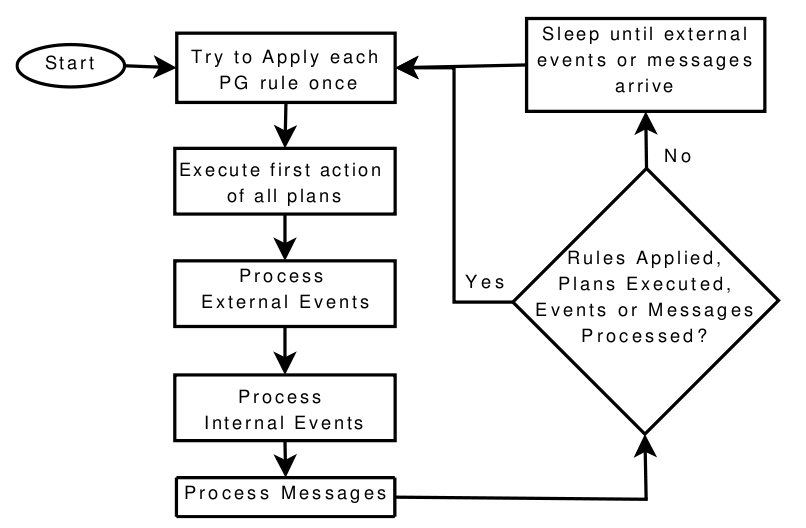
\includegraphics[keepaspectratio,scale=0.35]{fig/rcycle.png}
\caption{Predefined deliberation Cycle}
\label{fig:deliberation_cycle}
\end{figure}
 
Each cycle starts by applying all applicable PG-rules, each rule only one time. The deliberation cycle proceeds by executing only the first actions of all plans. This is in order to allow all plans to get a chance to be executed. The next deliberation steps are to
process all events received from the external environment, all internal events indicating the failure of plans, and all messages received from other agents, respectively. An event from external environment is processed by applying the first applicable PC-rule to it. An internal event, which identifies a failed plan, is processed by applying the first applicable PR-rule to the failed plan. A received message is then processed by applying the first applicable PC-rule to it. It is worth noting that the application of rules
to process events generates and add plans to the corresponding agent’s plan base.

If in a deliberation cycle no rule could be applied, no plan could be executed, and no event could be processed, then it makes no sense to try again a new cycle of deliberation steps, except when a new event or message has arrived.

The predefined deliberation cycle has the two following properties: first, if the execution of a plan fails, then the plan will either be repaired in the same deliberation cycle or get re-executed in the next deliberation cycle, since plans are executed before internal events are processed. Second, if the first action fails and there is no plan repair rule for it, then the failed plan may be successfully executed in the next deliberation cycle, since the belief and a goal bases can be modified in one deliberation cycle such that belief and goal test actions may be executed successfully in the next cycle.


\section{Conclusion} %%%%%%% BORJA HERE

%Borja here: conclusion + connecting with other alternatives (jadex etc)

\section{Bibliography}
\nocite{*}
\bibliographystyle{plain}
\bibliography{2apl-doc}

\end{document}
